%elatex
\documentclass[a4paper, 12pt, oneside]{extarticle}
%hell-escape
\input{~/Templates/lpnu_doc_templates/settings/preamble.tex}

\newcommand\Variant{4}
\newcommand\Date{03.03.\the\year}
\newcommand\Discipline{Алгоритмізація та програмування, частина 2}
\newcommand\Instructor{Кулешник Я. Ф.}

\newcommand\Work{\Lab~\No1}
\newcommand\Type{\Lab}
\newcommand\Number{1}
\newcommand\Topic{Машина Поста}

\begin{document}
\Margins

\Margins
%\begin{wrapfigure}[3]{l}{.27\textwidth}
%\includegraphics[width=.28\textwidth]{$UNI/.templates/lpnu_logo.png}
%\end{wrapfigure}

%\noindent\textbf{Прізвище:} \Lname \\
%\noindent\textbf{Ім'я:} \Fname \\
%\noindent\textbf{Група:} \Group \\
%\noindent\textbf{Варіант:} \Variant \\
%\noindent\textbf{Дата захисту:} \Date \\
%\\
%\noindent\textbf{Кафедра:} \Department \\
%\noindent\textbf{Дисципліна:} \Discipline \\
%\noindent\textbf{Перевірив:} \Instructor \\

%%\medskip\bigskip

%\begin{center}
%	\textbf{ЗВІТ}		\\
%	до \Type~\No\Number	\\
%	на тему ``\Topic''	\\
%\end{center}

% \begin{table}
%   \begin{tabularx}{\textwidth}{|c|X|X|}
%     \hline
%     % Image & Content & Additional Info \\
%     % \hline
% 	  \multirow{3}{*}{\includegraphics[width=4cm]{$UNI/.templates/lpnu_logo.png}}
% 	  & \textbf{ЗВО:}
% 	  Національний університет ``Львівська Політехніка''.
% 	  & \textbf{Тема:}
% 	  \Topic
% 	  \\
% 	  & \textbf{Навчальний рік:}
% 	  2023/2024
% 	  & \textbf{Інститут}
% 	  комп'ютерних наук та інформаційних технологій
% 	  \\
% 	  & \textbf{Семестр:}
% 	  осінній
% 	  & \textbf{Група:}
% 	  \Group
% 	  \\
% 	  & \textbf{Навчальна дисципліна:}
% 	  \Discipline
% 	  & \textbf{Студент:}
% 	  Мілюхін Олександр
% 	  \\
% 	  & \textbf{Кафедра}
% 	  систем автоматизованого проектування
% 	  &
% 	  \\
% 	  & \textbf{Викладач:}
% 	  Чумакевич В. В.
% 	  &
% 	  \\
%     \hline
%   \end{tabularx}
% \end{table}

\setlength{\textfloatsep}{-16pt}
% \setlength{\intextsep}{0pt}

\begin{table}
	\begin{tabular}{|l|l|p{6cm}|}
    \hline
    % Image & Content & Additional Info \\
    % \hline
	  \makecell[l]{
	  \includegraphics[width=3.37cm]{$UNI/.templates/lpnu_logo.png}
  }
	  & \makecell[l]{
	  \textbf{ЗВО:}
	  Національний університет \\ ``Львівська Політехніка''.
	  \\
	  \textbf{Навчальний рік:}
	  2023/2024
	  \\
	  \textbf{Семестр:}
	  осінній
	  \\
	  \textbf{Навчальна дисципліна:} \\
	  \Discipline
	  \\
	  \textbf{Кафедра}
	  систем автоматизованого \\ проектування
	  \\
	  \textbf{Викладач:}
	  Чумакевич В. В.
}
	  & \makecell [l] {
	  \textbf{Тема:}
	  \Topic
	  \\
          \textbf{Інститут}
	  комп'ютерних наук та \\ інформаційних технологій
	  \\
	  \textbf{Група:}
	  \Group
	  \\
	  \textbf{Студент:}
	  Мілюхін Олександр
  }
  \\
    \hline
  \end{tabular}
\end{table}
\section{Мета роботи}

% \begin{table}
%   \begin{tabularx}{\textwidth}{|p{6cm}|c|c|}
% 	  \hline
%     \multirow{3}{*}{\includegraphics[width=6cm]{$UNI/.templates/lpnu_logo.png}}
% 	  & ЗВО: Національний університет ``Львівська Політехніка''
% 	  & Additional Info 1 \\
%     & Content 2 & Additional Info 2 \\
%     & Content 3 & Additional Info 3 \\
% 	  \hline
%   \end{tabularx}
% \end{table}

% \begin{table}
%   \begin{tabular}{|c|c|c|}
%     \hline
%     \multirow{3}{*}{\includegraphics[width=3cm]{$UNI/.templates/lpnu_logo.png}} & \makecell{Content 1 \\ Content 2 \\ Content 3} & \makecell{Additional Info 1 \\ Additional Info 2 \\ Additional Info 3} \\
%     \hline
%   \end{tabular}
% \end{table}


Мета роботи – вивчення формального визначення поняття алгоритму,
пов’язаного із введеною Емілем Постом спеціальної математичної
конструкції (машина Поста) і постулюванням тези про еквівалентність

\subsubsection*{Завдання}

Скласти програму додавання 2-х цілих додатних чисел а і b,
розташованих на стрічці машини Поста. Каретка розташована над
однією з міток, що належать числу а. Число b знаходиться правіше за
число а через декілька порожніх комірок.

%---------------------------------------------
\section*{Етапи розв'язку}

\subsection*{Блок-схема алгоритму}

\begin{figure}[h]
	\centering
	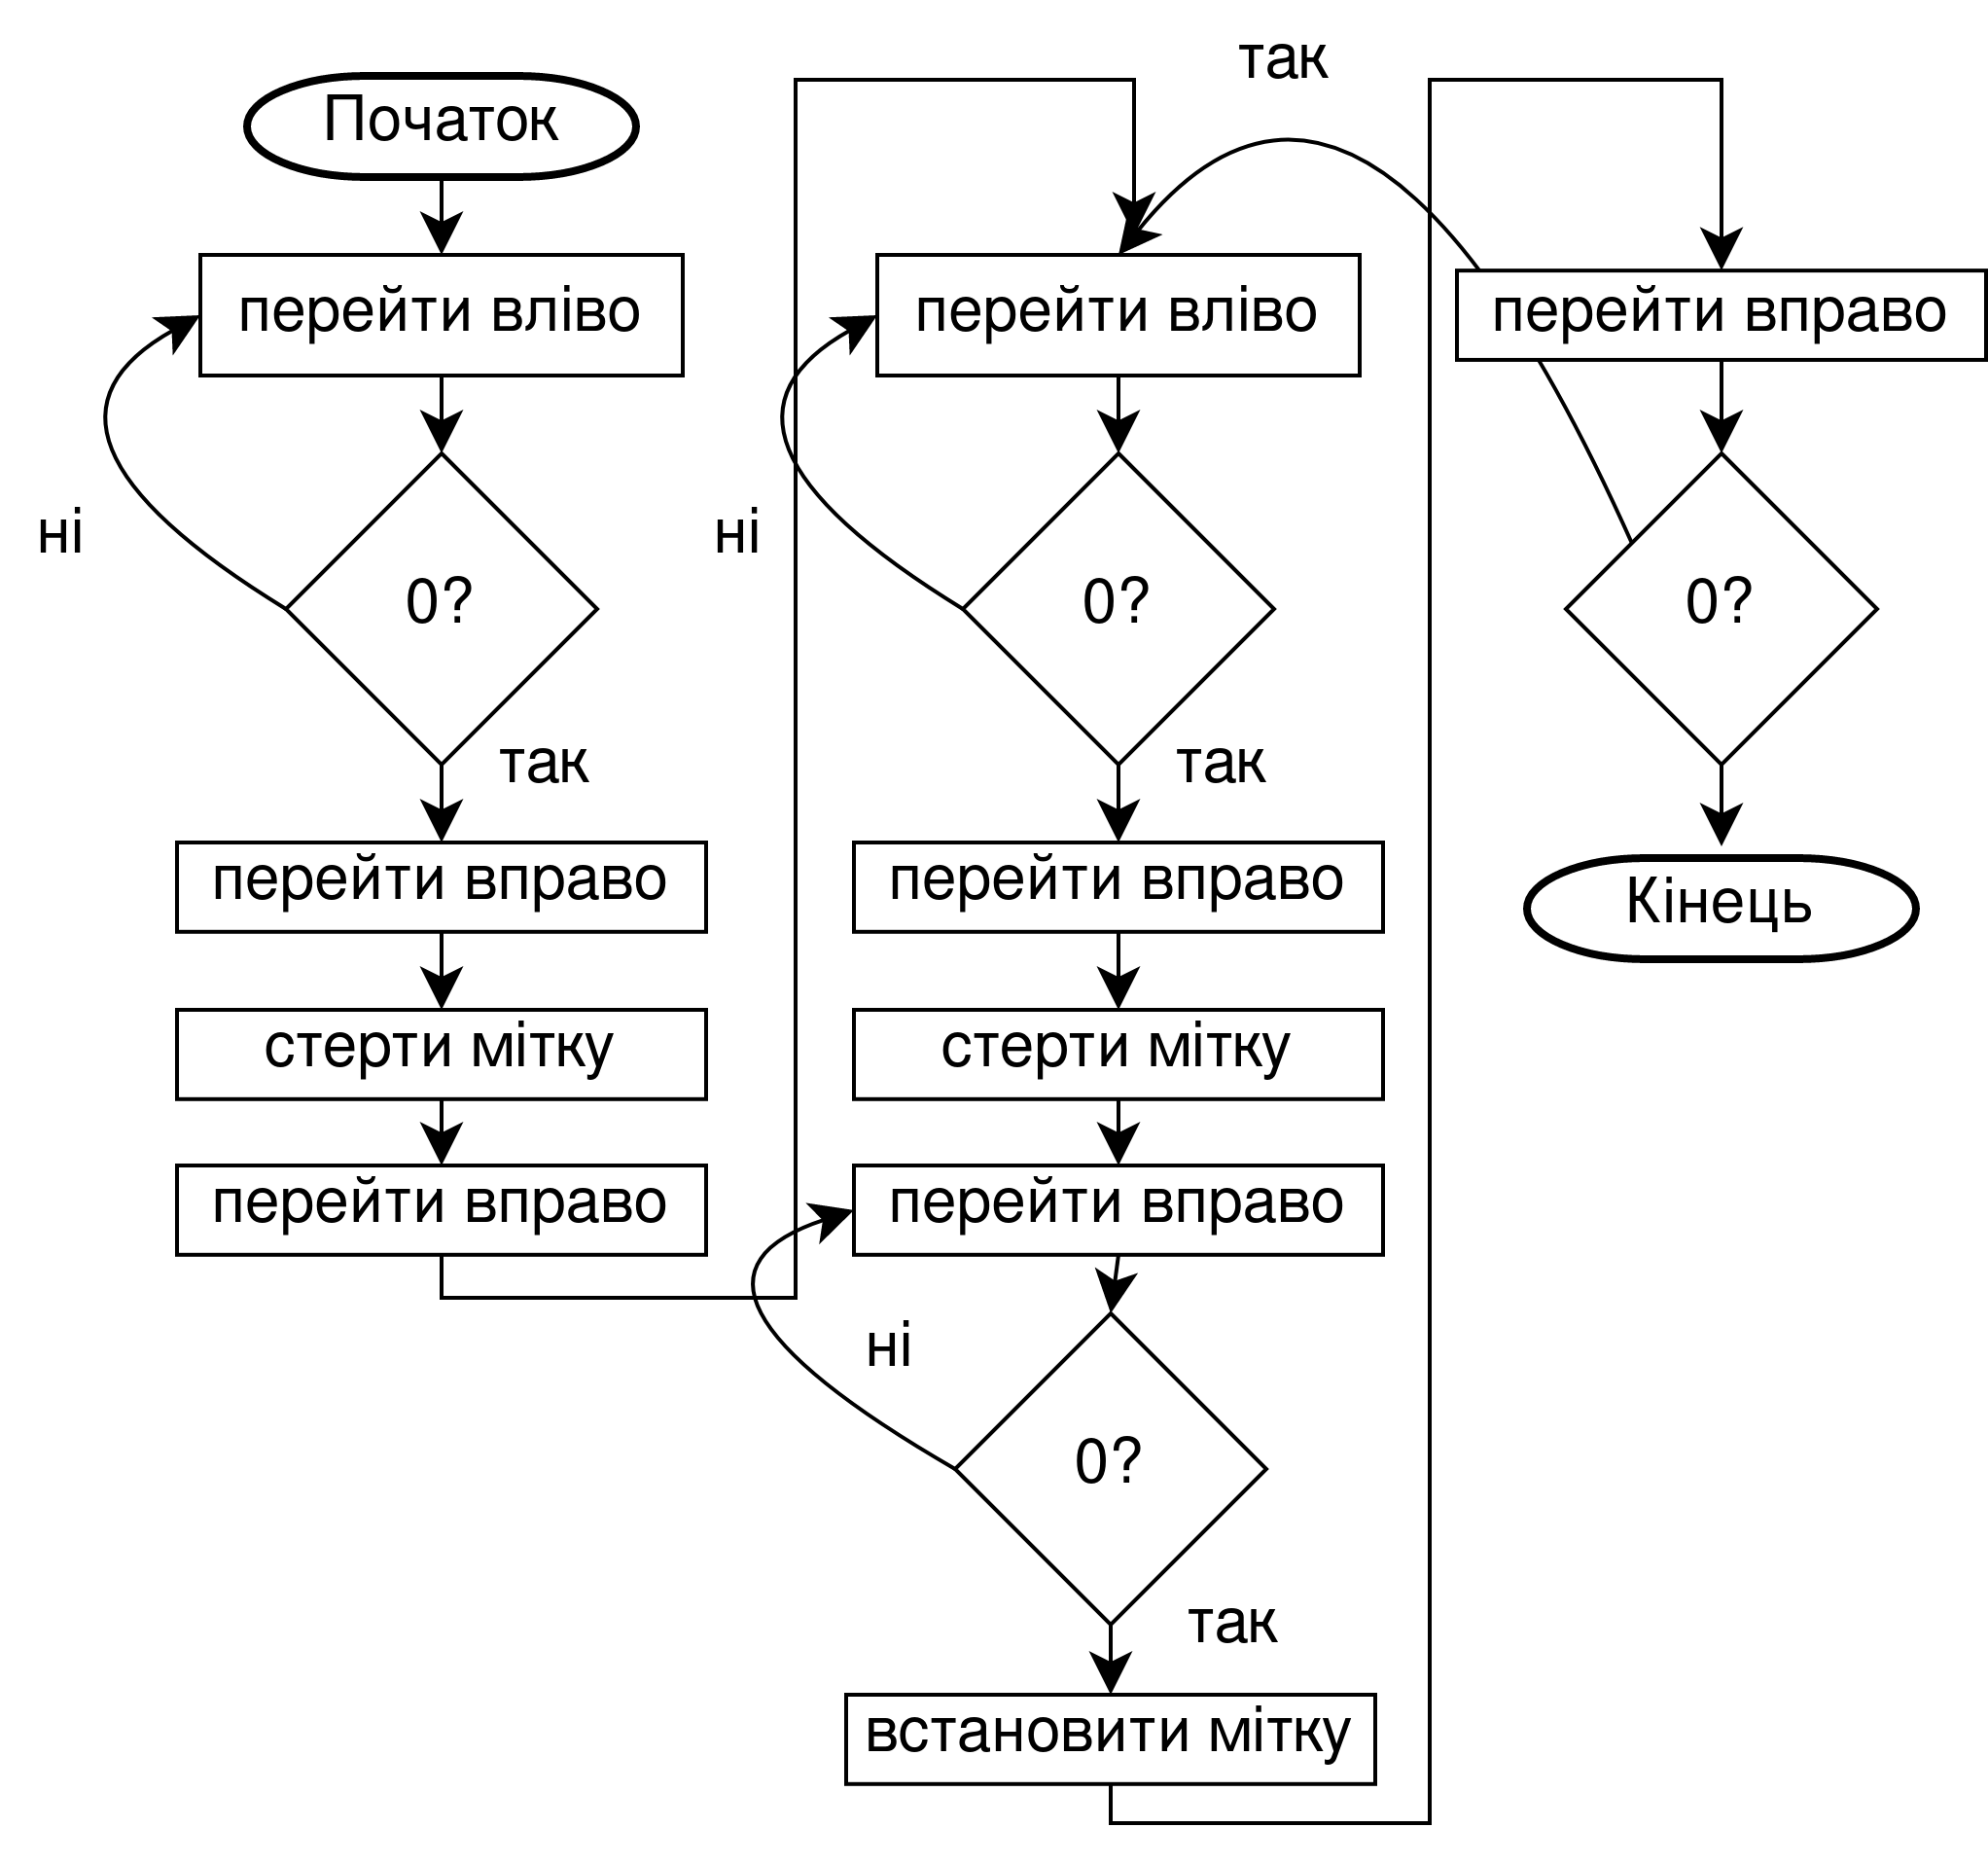
\includegraphics[width=.6\textwidth]{diag.png}
\end{figure}

\subsection*{Код програми}

\verbatiminput{./command_list.txt}
\listinginput{1}{./1.cpp}
%\verbatiminput{1.cpp}
%\lstinputlisting[frame=single, firstline=1]{./1.cpp}

\subsection*{Вхідні дані}
\verbatiminput{tape.txt}

\subsection*{Результат виконання програми}

\verbatiminput{result.txt}

\subsection*{Висновок}

Виконуючи цю лабораторну роботу, я навчився писати
невеликі програми для машини Поста.

У процесі роботи
я натрапив на легкий емулятор машини Поста з інтерфейсом
командного рядка і, переконавшись у його зручності, завершив
виконання роботи в ньому.

Щодо завдання, бачимо, що два числа дійсно були додані з урахуванням зайвого нуля,
який програма прибрала на початку виконання.

\subsection*{Відповіді на контрольні запитання}
\begin{enumerate}
	\item	Що постулює так звана «теза Поста»?

		Будь-який алгоритм можна представити як програму для машини Поста.

	\item	Що таке алгоритм за Постом?

		Алгоритм за Постом --- програма для машини Поста, що приводить до виконання
		поставленої задачі.

	\item	Що таке машина Поста?

	Машина Поста – це абстрактна (тобто така, що не існує в арсеналі
	техніки), але дуже проста обчислювальна машина.

	\item	Які складові абстрактної машини Поста?

Машина Поста складається із стрічки та каретки (яка також
називається головкою зчитування/запису). Стрічка є безмежною і розділена
на однакові комірки.

	\item	Який набір команд виконує машина Поста?

		\begin{itemize}

	\item	Записати мітку й перейти до вказаного рядка
	\item	Записати 0 і перейти до вказаного рядка
	\item	переміститись управо й перейти до вказаного рядка
	\item	переміститись уліво й перейти до вказаного рядка
	\item	зупинка
	\item	0? перейти до вказаного рядка

		\end{itemize}

	\item	Що таке початковий стан каретки?

		Її початкове положення відносно стрічки.

	\item	Що таке стан стрічки?

		Інформація про те, які комірки містять мітки, а які ні.

	\item	Що таке стан машини Поста?

		Стан стрічки й каретки.

	\item	Навести перелік неприпустимих дій, які ведуть до аварійної зупинки машини.

		\begin{itemize}

	\item	спроба записати 1 (мітку) в заповнену комірку;
	\item	спроба стерти мітку в порожній комірці;
	\item	нескінченне виконання (зациклення).

		\end{itemize}

	\item	Що таке програма для машини Поста?

	Програмою для машини Поста називається непорожній список
	послідовно пронумерованих команд наступної структури: n K m, де n -
	порядковий номер команди, K --- дія, яка виконується кареткою, m - номер
	наступної команди, яку необхідно

	\item	Коли програма застосовна до біжучого стану машини Поста?

		Коли виконання програми не призведе до
		зациклювання, тобто рано чи пізно ми виконаємо команду «Зупинка».

\end{enumerate}

\end{document}

\footnotesize
\begin{multicols}{4}
\begin{verbatim}
Tape states:
          V
..0000001111100001..
          V
..0000000111110000..
          V
..0000000111110000..
          V
..0000000011111000..
          V
..0000000011111000..
          V
..0000000001111100..
          V
..0000000001111100..
          V
..0000000011111000..
          V
..0000000001111000..
          V
..0000000011110000..
          V
..0000000001111000..
          V
..0000000001111000..
          V
..0000000011110000..
          V
..0000000001110000..
          V
..0000000011100001..
          V
..0000000011100001..
          V
..0000000111000011..
          V
..0000000111000011..
          V
..0000001110000111..
          V
..0000001110000111..
          V
..0000011100001110..
          V
..0000011100001110..
          V
..0000011110001110..
          V
..0000111100011100..
          V
..0000111100011100..
          V
..0000011110001110..
          V
..0000011110001110..
          V
..0000001111000111..
          V
..0000001111000111..
          V
..0000000111100011..
          V
..0000000111100011..
          V
..0000000011110001..
          V
..0000000011110001..
          V
..0000000001111000..
          V
..0000000001111000..
          V
..0000000011110001..
          V
..0000000001110001..
          V
..0000000011100011..
          V
..0000000011100011..
          V
..0000000111000111..
          V
..0000000111000111..
          V
..0000001110001110..
          V
..0000001110001110..
          V
..0000011100011100..
          V
..0000011100011100..
          V
..0000011110011100..
          V
..0000111100111000..
          V
..0000111100111000..
          V
..0000011110011100..
          V
..0000011110011100..
          V
..0000001111001110..
          V
..0000001111001110..
          V
..0000000111100111..
          V
..0000000111100111..
          V
..0000000011110011..
          V
..0000000011110011..
          V
..0000000001111001..
          V
..0000000001111001..
          V
..0000000011110011..
          V
..0000000001110011..
          V
..0000000011100111..
          V
..0000000011100111..
          V
..0000000111001110..
          V
..0000000111001110..
          V
..0000001110011100..
          V
..0000001110011100..
          V
..0000011100111000..
          V
..0000011100111000..
          V
..0000011110111000..
          V
..0000111101110000..
          V
..0000111101110000..
          V
..0000011110111000..
          V
..0000011110111000..
          V
..0000001111011100..
          V
..0000001111011100..
          V
..0000000111101110..
          V
..0000001110111000..
          V
..0000001110111000..
          V
..0000011101110000..
          V
..0000011101110000..
          V
..0000011111110000..
          V
..0000111111100000..
          V
..0000111111100000..
\end{verbatim}
\end{multicols}{4}

\normalsize
